\documentclass[14pt]{extarticle}
\usepackage[utf8]{inputenc}
\usepackage[T1]{fontenc}
\usepackage[spanish,es-lcroman]{babel}
\usepackage{amsmath}
\usepackage{amsthm}
\usepackage{physics}
\usepackage{tikz}
\usepackage{float}
\usepackage[autostyle,spanish=mexican]{csquotes}
\usepackage[per-mode=symbol]{siunitx}
\usepackage{gensymb}
\usepackage{multicol}
\usepackage{enumitem}
\usepackage[left=2.00cm, right=2.00cm, top=2.00cm, 
     bottom=2.00cm]{geometry}
\usepackage{Estilos/ColoresLatex}

\newcommand{\textocolor}[2]{\textbf{\textcolor{#1}{#2}}}

%\renewcommand{\questionlabel}{\thequestion)}
\decimalpoint
\sisetup{bracket-numbers = false}

\title{\vspace*{-2cm} Ejercicios Opcionales - Física 1\vspace{-5ex}}
\date{\today}

\begin{document}
\maketitle

\section{Ejercicios a cuenta}

Con la finalidad de apoyar en la recuperación del promedio para los siguientes exámenes parciales, se dejarán una serie de \textocolor{red}{ejercicios adicionales} para Evaluación Continua.


Estos ejercicios serán de carácter \textocolor{cobalt}{opcional}, es decir, la alumna o alumno que desee resolverlos y enviarlos, les sumará $5$ puntos adicionales a la Evaluación Continua.

La entrega se hará vía Teams en asignación, teniendo como plazo el día domingo 16 de julio a las 8 pm.

Cada ejercicio vale $1$ punto, siempre y cuando esté correcto. Se otorgará una parte proporcional en caso de tener desarrollo detallado pero el resultado no sea el esperado.

Anota en la hoja tu nombre completo, así como una identificación de cada ejercicio.

\begin{enumerate}
\item Encuentra la velocidad media o promedio de un automóvil que durante su recorrido hacia el norte tuvo las
siguientes magnitudes de velocidades:
\begin{align*}
v_{1} &= \SI{18.5}{\meter\per\second}, \hspace{0.5cm} v_{2} = \SI{22}{\meter\per\second} \\[0.5em]
v_{3} &= \SI{20.3}{\meter\per\second}, \hspace{0.5cm} v_{4} = \SI{21.5}{\meter\per\second}
\end{align*}
\item Un automóvil parte del reposo y experimenta una aceleración cuya magnitud es de \SI{1.5}{\meter\per\square\second}. ¿Qué distancia habrá recorrido después de \SI{2}{\second}?
\item Un avión vuela en la misma dirección y sentido a \SI{860}{\kilo\meter\per\hour} durante un tiempo de \SI{20}{\minute}. ¿Cuál es su aceleración durante ese intervalo de tiempo y por qué?
\item En la siguiente gráfica se muestra la posición en función del tiempo para cierto objeto que se mueve a lo largo del eje $x$.
\begin{figure}[H]
    \centering
    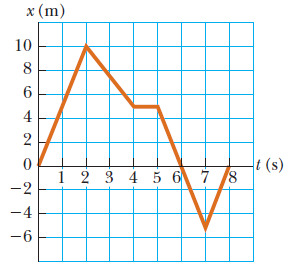
\includegraphics[scale=1]{Imagenes/Ejercicio_Cuenta_01.png}
\end{figure}
Encuentra la velocidad en los siguientes intervalos de tiempo:
\begin{enumerate}[label=\alph*)]
\item \num{0} a \SI{2}{\second}
\item \num{0} a \SI{4}{\second}
\item \num{2} a \SI{4}{\second}
\item \num{4} a \SI{7}{\second}
\item \num{0} a \SI{8}{\second}
\end{enumerate}
\item Determina la velocidad que llevará un muchacho en su patineta a los \SI{6}{\second}, si al bajar por una pendiente adquiere una aceleración cuya magnitud es de \SI{0.7}{\meter\per\square\second} y parte con una velocidad inicial de \SI{4}{\meter\per\second}.
\end{enumerate}

\end{document}